%
% Capítulo 4
%
\chapter{Architecture} \label{cap:architecture}

This chapter provides an overview of the system’s components and their interactions.
It outlines the capabilities of the project and presents the architecture, entities, and
implementation blueprint that have been designed and developed.

\section{Overview}

Figure ~\ref{fig:architecture} presents a diagram illustrating the main components of the system and their interactions. The system consists of a backend application (server-side) and a frontend application (client-side).
The backend comprises a collection of services, responsible for data manipulation and storage database.
The frontend is composed of a web application, that facilitates user interaction. Communication between the frontend and the backend is achieved through a REST API, utilizing the HTTP protocol [24].

\begin{figure}[H]
	\begin{center}
		\resizebox{150mm}{!}{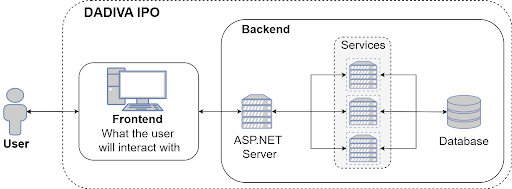
\includegraphics{./figures/Architecture.png}}
	\end{center}
	\caption{Application Architecture.}\label{fig:architecture}
\end{figure}

\section{Form Data Model}

The first approach to solve de dynamic form challenge was to use a data structure formed by main questions and sub-questions, example presented in Figure ~\ref{fig:old_form}, where a main question can only be answered with boolean values, and one of those values triggers the display of a sub-question which has a certain type of response, such as boolean, dropdown for known multiple answers, and text to accept user text input.


\begin{figure}[hbt!]
	\begin{center}
		\resizebox{150mm}{!}{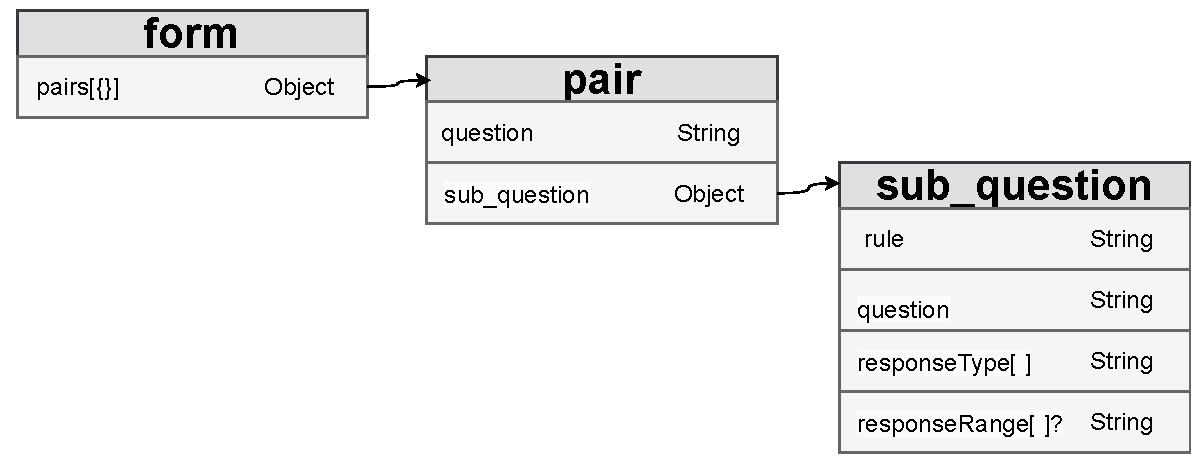
\includegraphics{./figures/oldForm.pdf}}
	\end{center}
	\caption{First Form Data Structure.}\label{fig:old_form}
\end{figure}

This approach has some drawbacks, such as the fact that it disables the possibility of supressing further questions, hence not adhering to the principle of creating a generic and adaptable solution, and mixes questions and rules in the sub-question.

Upon further discussion we settled on using a more complex data structure , exemplified in Figure ~\ref{fig:new_form}, composed by a list of questions and a list of rules.

Each question has an id, the text that composes it, the type of response (boolean, text and dropdown) and can have options that lists all the possibles values for a multiple(dropdown) response.

Each rule has conditions, which can be "any","all" or "not", so that, when any, all or none of the conditions are met an event is triggered, which can be to show or hide a question, the question targeted by the event is identified by the id, supplied via the params field.


\begin{figure}[htbp]
	\begin{center}
		{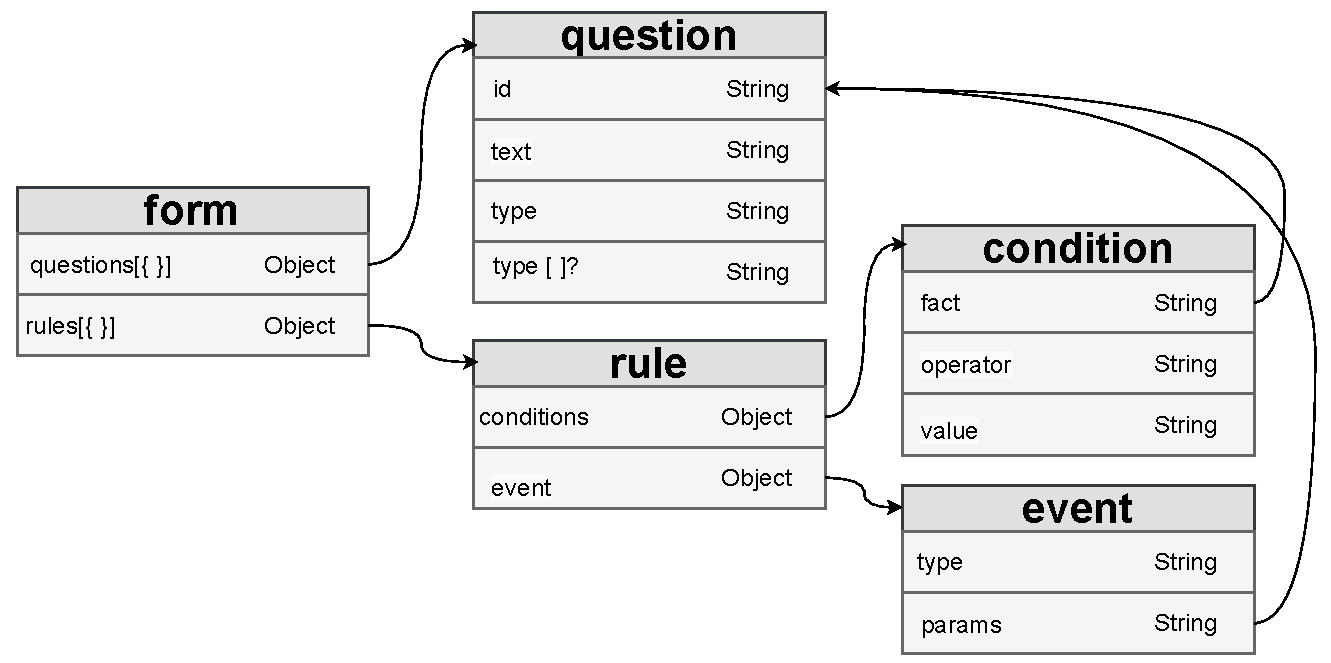
\includegraphics[width=\textwidth,height=\textheight,keepaspectratio]{./figures/newForm.pdf}}
	\end{center}
	\caption{Final Form Data Structure.}\label{fig:new_form}
\end{figure}
\FloatBarrier


\section{Frontend Application}

The frontend application is composed of a web application, which is responsible for the interaction between the users and the backend. This application provides a simple and intuitive interface for the user to interact with the system, allowing donor users to fill out the current form, doctor users to search for pathology and medication interaction with blood donation and request form answers of a given user and administrator users to customize the current form, update the pathology and medication interaction information and manage the user.
This application is divided into multiple pages and components, and has a service
layer that is responsible for communicating with the backend application through the
REST API.

\section{Services}

The backend application is composed of a set of services, responsible for data manipulation and storage. Each service is associated with a given domain and is independent from the remaining services, allowing for ease of future updates.
The services communicate with the database, in which the various data models are divided into specific indexes, such as:

\begin{itemize}
	\item /form: stores all the forms ;
	\item /submissions: stores all the user form responses ;
	\item /users: stores all the users.
\end{itemize}

The system is composed of the following services:

\begin{itemize}
	\item form: responsible for form management, such as, creation, requests, submission, editing and deletion;
	\item search: responsible for medication and pathology interaction information management;
	\item users: responsible for user management, such as, registration, login, deletion and role management.
\end{itemize}

\subsection{Form Services}

The form service is responsible for managing the form resources.
Figure ~\ref{fig:form_services} is a diagram that shows the architecture of the form services.

\begin{figure}[htbp]
	\begin{center}
		\resizebox{150mm}{!}{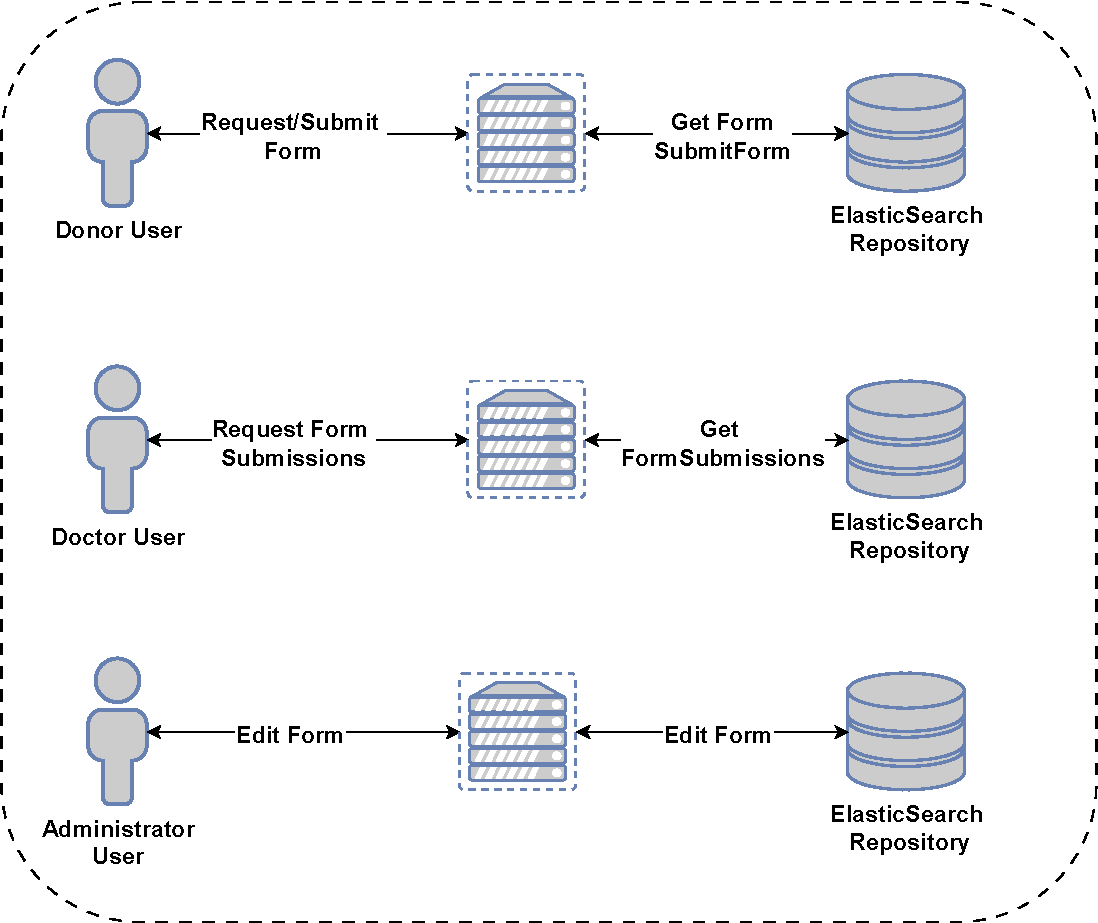
\includegraphics{./figures/formServices.pdf}}
	\end{center}
	\caption{Final Form Data Structure.}\label{fig:form_services}
\end{figure}
